%%%%%%%%%%%%%%%%%%%%%%%%%%%%%%%%%%%%%%%%%
% University/School Laboratory Report
% LaTeX Template
% Version 3.1 (25/3/14)
%
% This template has been downloaded from:
% http://www.LaTeXTemplates.com
%
% Original author:
% Linux and Unix Users Group at Virginia Tech Wiki 
% (https://vtluug.org/wiki/Example_LaTeX_chem_lab_report)
%
% License:
% CC BY-NC-SA 3.0 (http://creativecommons.org/licenses/by-nc-sa/3.0/)
%
%%%%%%%%%%%%%%%%%%%%%%%%%%%%%%%%%%%%%%%%%

%----------------------------------------------------------------------------------------
%	PACKAGES AND DOCUMENT CONFIGURATIONS
%----------------------------------------------------------------------------------------

\documentclass{article}

\usepackage[version=3]{mhchem} % Package for chemical equation typesetting
\usepackage{siunitx} % Provides the \SI{}{} and \si{} command for typesetting SI units
\usepackage{graphicx} % Required for the inclusion of images
\usepackage{natbib} % Required to change bibliography style to APA
\usepackage{amsmath} % Required for some math elements 
\usepackage{gensymb}

\setlength\parindent{0pt} % Removes all indentation from paragraphs

\renewcommand{\labelenumi}{\alph{enumi}.} % Make numbering in the enumerate environment by letter rather than number (e.g. section 6)

%\usepackage{times} % Uncomment to use the Times New Roman font


%Code packages

\usepackage[utf8]{inputenc}
\usepackage{listings}
\usepackage{color}
% Code packages end


%----------------------------------------------------------------------------------------
%	DOCUMENT INFORMATION
%----------------------------------------------------------------------------------------

\title{Ising Ferro-magnetism\\ PHY 230} % Title

\author{Avi \textsc{Vajpeyi}} % Author name

\date{\today} % Date for the report

\begin{document}

\maketitle % Insert the title, author and date



% If you wish to include an abstract, uncomment the lines below
% \begin{abstract}
% Abstract text
% \end{abstract}

%----------------------------------------------------------------------------------------
%	SECTION 1
%----------------------------------------------------------------------------------------

\section{Theory and Insights from the App }

The theory for this project was interesting as I had not known of the Ising Model before this class. I knew that ferro-magnets had spins in them, however did not know that we had discovered a way to model the spins of ferro-magnets at different temperatures.

It was interesting to see that at the Curie temperature, the up and down spins seemed to balance each other, and even more interestingly, there seemed to be clumps of space with up spins, and clumps of space with down spins. Each of the clumps seemed to have the other spin in it as well, speckled through out the clump (i.e the up spin clumps had down spins randomly situated inside the clump). This can be seen in fig~\ref{CurieTemp}.






\begin{figure}[h]
	\caption{Picture of the spins at the Curie temperature. }
	\centering
	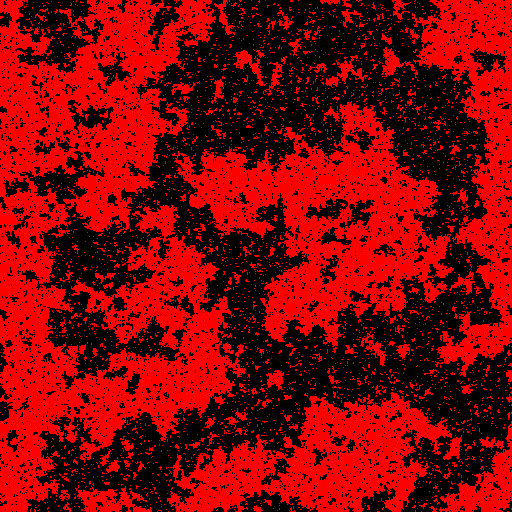
\includegraphics[width=0.5\textwidth]{CurieTemp} \label{CurieTemp}
\end{figure}

 At other temperatures above the curie temperature, there appeared to be an equal number of up and down spins, however no clumping was present, as seen in fig~\ref{higherTemp}. In a way, there were small clumps, but not like the clumps present at the curie temperature. At these higher temperatures, the ferro magnet's spins looked like the static on a cathode ray TV screen. 



\begin{figure}[h]
	\caption{Picture of the spins at a high temperature of 5.}
	\centering
	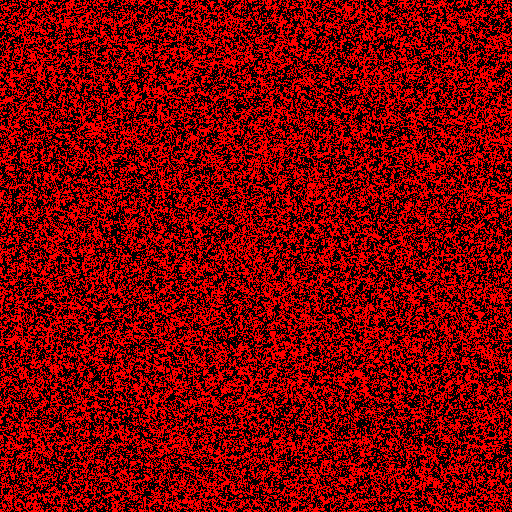
\includegraphics[width=0.5\textwidth]{HighTemp} \label{higherTemp}
\end{figure}





In fig~\ref{lowTemp} we can see what the model of the spins looks like at temperatures below the curie temperature. Here, the spins seem to clump up the most, with the least amount of specks of the opposite spin in side the clumps. I think that at this point, where the majority of the spin is in one direction, the ferromagnet will have a a higher amount of magnetism.



\begin{figure}[h]
	\caption{Picture of the spins at a low temperature of 1.}
	\centering
	
\includegraphics[width=0.5\textwidth]{LowTemp} \label{lowTemp}
\end{figure}

\section{Program and Data Analysis } 

We ran the app using a bitmap and without a bitmap. We realized that not using a bitmap made the program run at an amazingly slow rate. It became frustrating to use and slow. Saving data for 50 points with this method took 2.7 seconds while using the bitmap took 0.6 seconds. This made us realise how useful bitmaps can be. 

We ran tests in which we kept the temprature constant, at he curie temperature, and saved the normalised magnetisation and energy for 500 consecutive data points. Graphs that we created from this data can be seen in fig ~ \ref{Time}. From the graphs we can see that with time, the magnetisation increased while the energy decreased. This did not make sense to me - I expected that the energy and magnetisation would remain relatively the same, fluctuating about one region. 

  
  \begin{figure}[h]
  	\caption{Graphs of the normalised magnetisation and energy against the time in number of data points with constant temperature at the curie temperature.}
  	\centering
  	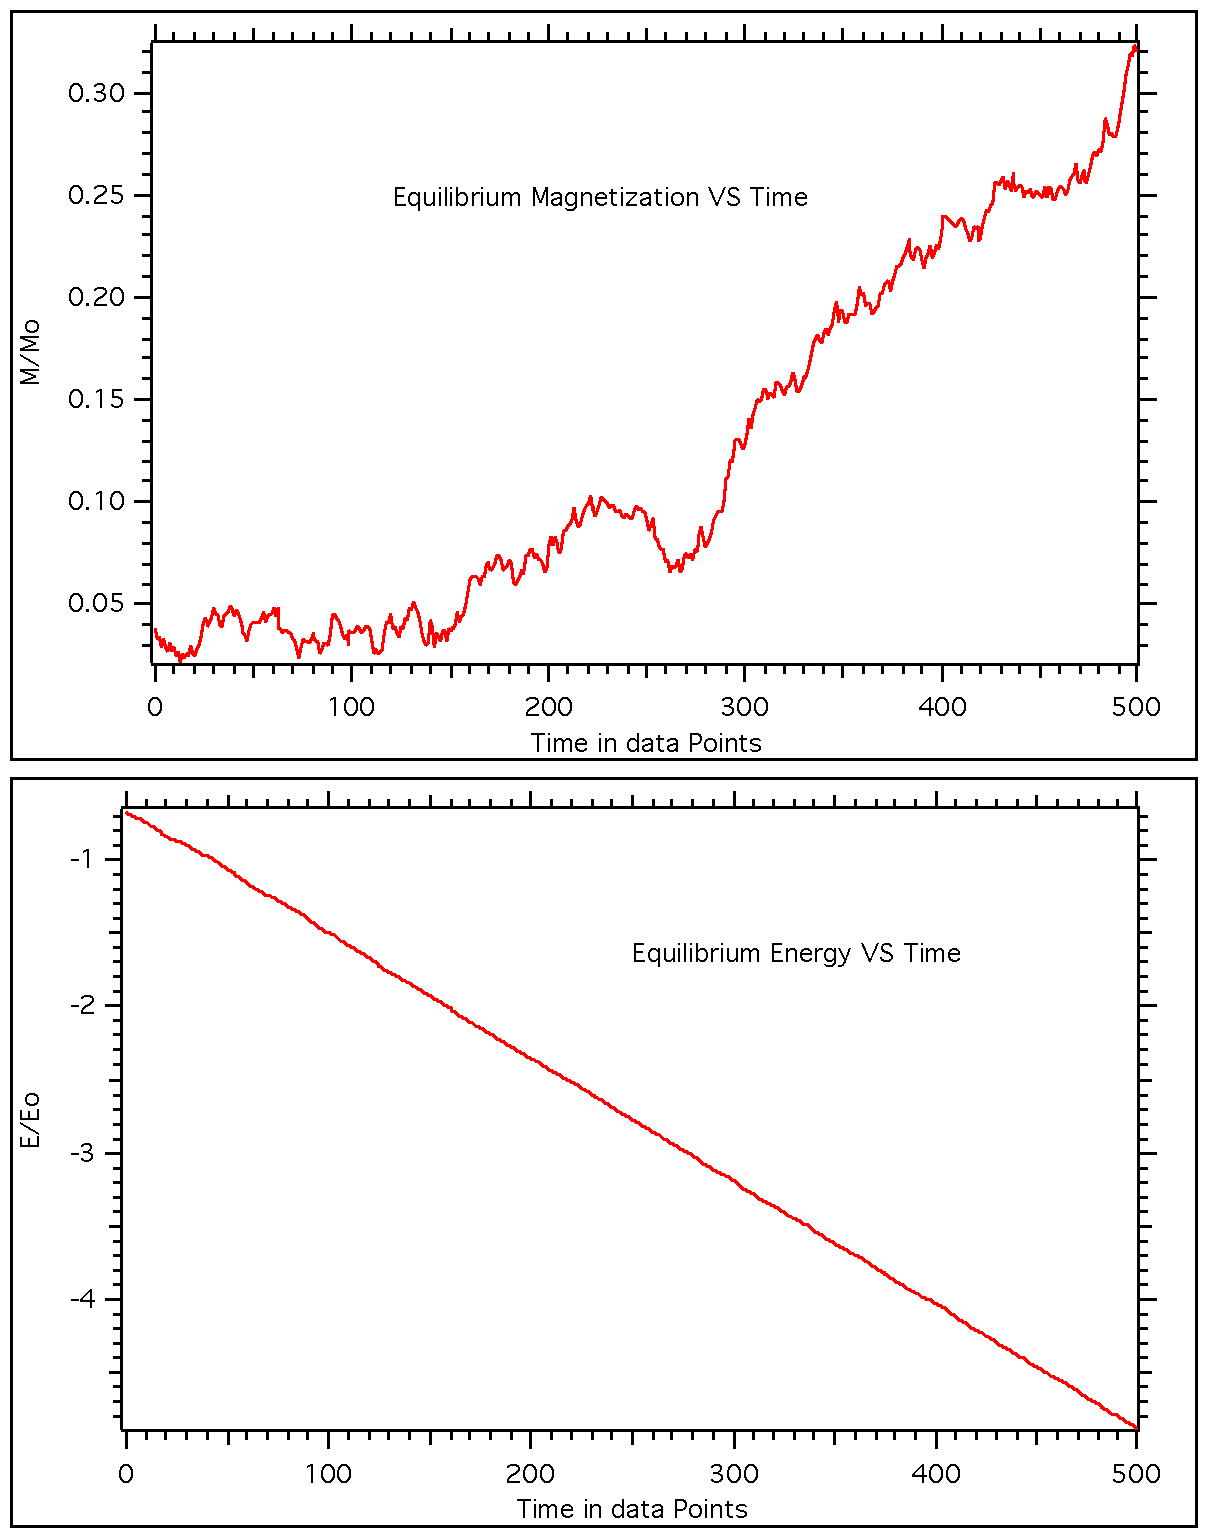
\includegraphics[width=0.5\textwidth]{Time} \label{Time}
  \end{figure}
  
  



Hence I decided to repeat the test, but for a longer duration. Fig~\ref{LongTime} shows the graphs of normalised magnetisation and energy against time for 1000 consecutive data points. This time we see that magnetisation and energy decrease with increase in time. This result, like the previous, is quite confusing to me. I tried to read up on it online, but was unable to understand what is happening here. Although I have not been able to make any conclusions from this, this has shown me why I need to take the EM class next semester. 

  \begin{figure}[h]
  	\caption{Graphs of the normalised magnetisation and energy against the time in number of data points with constant temperature at the curie temperature. The time for this graph is longer than that of fig~\ref{Time}.}
  	\centering
  	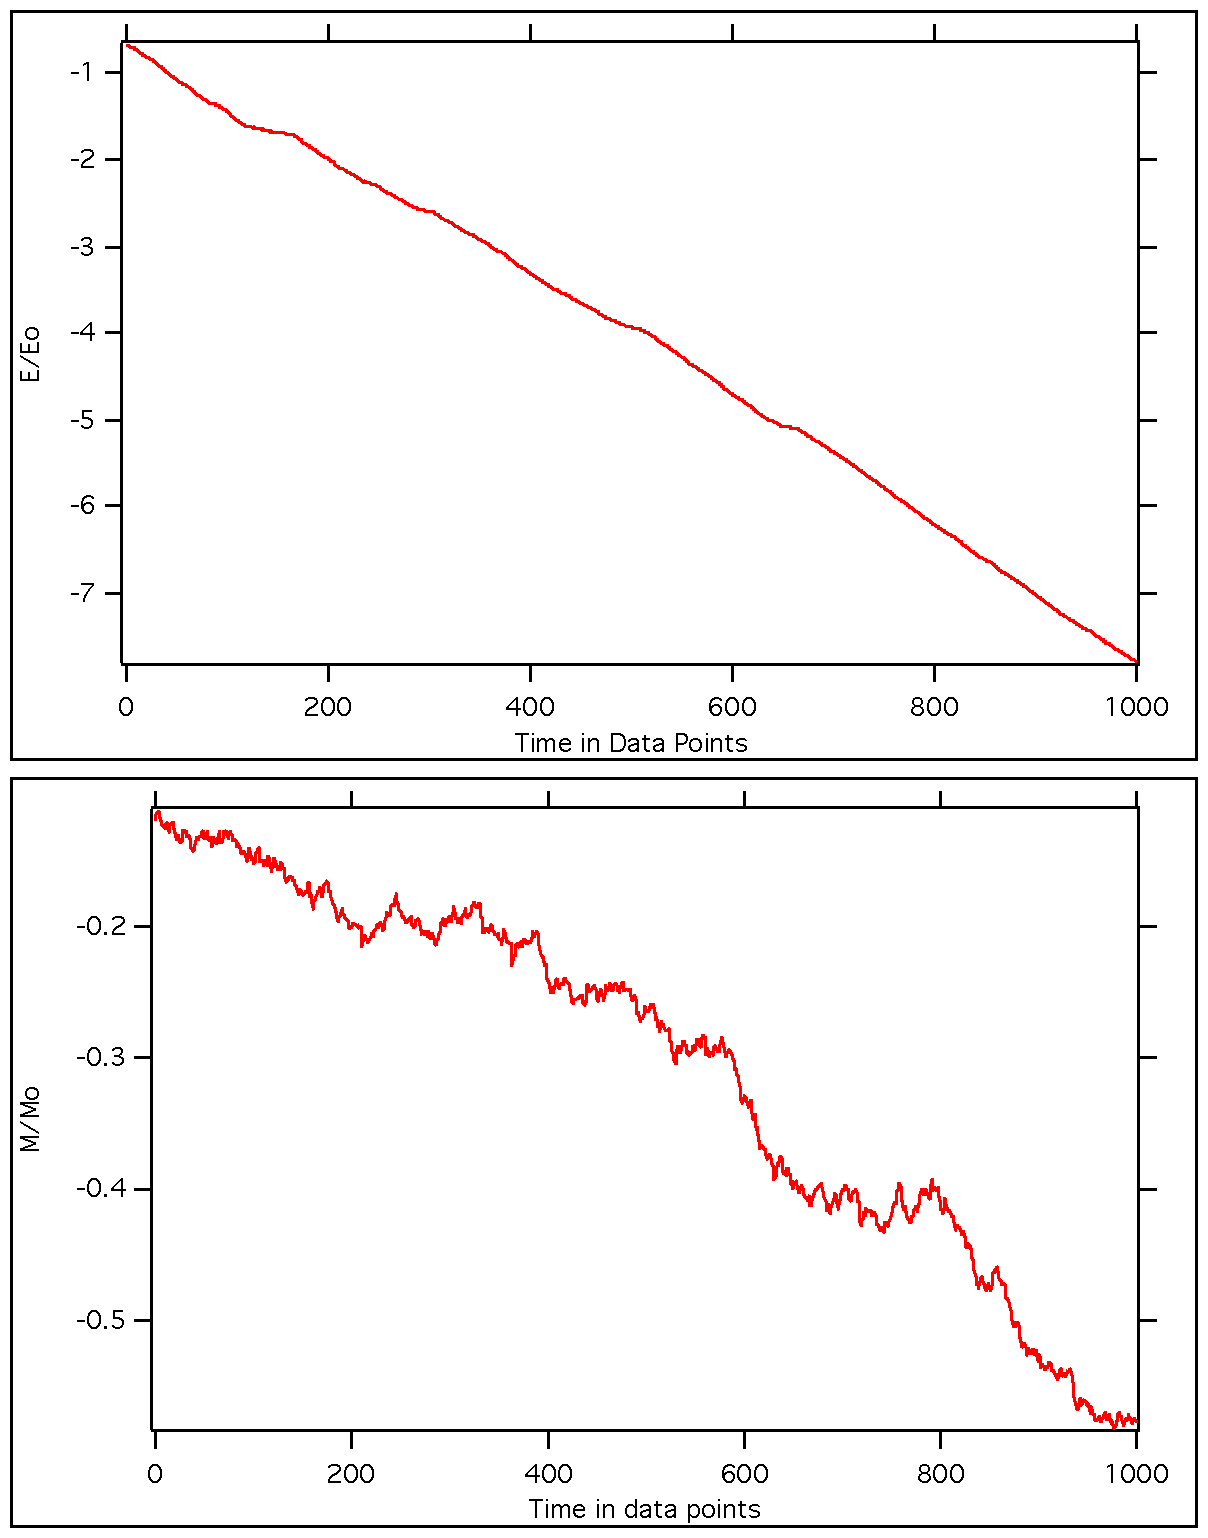
\includegraphics[width=0.5\textwidth]{TimeLong} \label{TimeLong}
  \end{figure}

  \begin{figure}[h]
  	\caption{Graphs of the normalised magnetisation and energy against the temperature.}
  	\centering
  	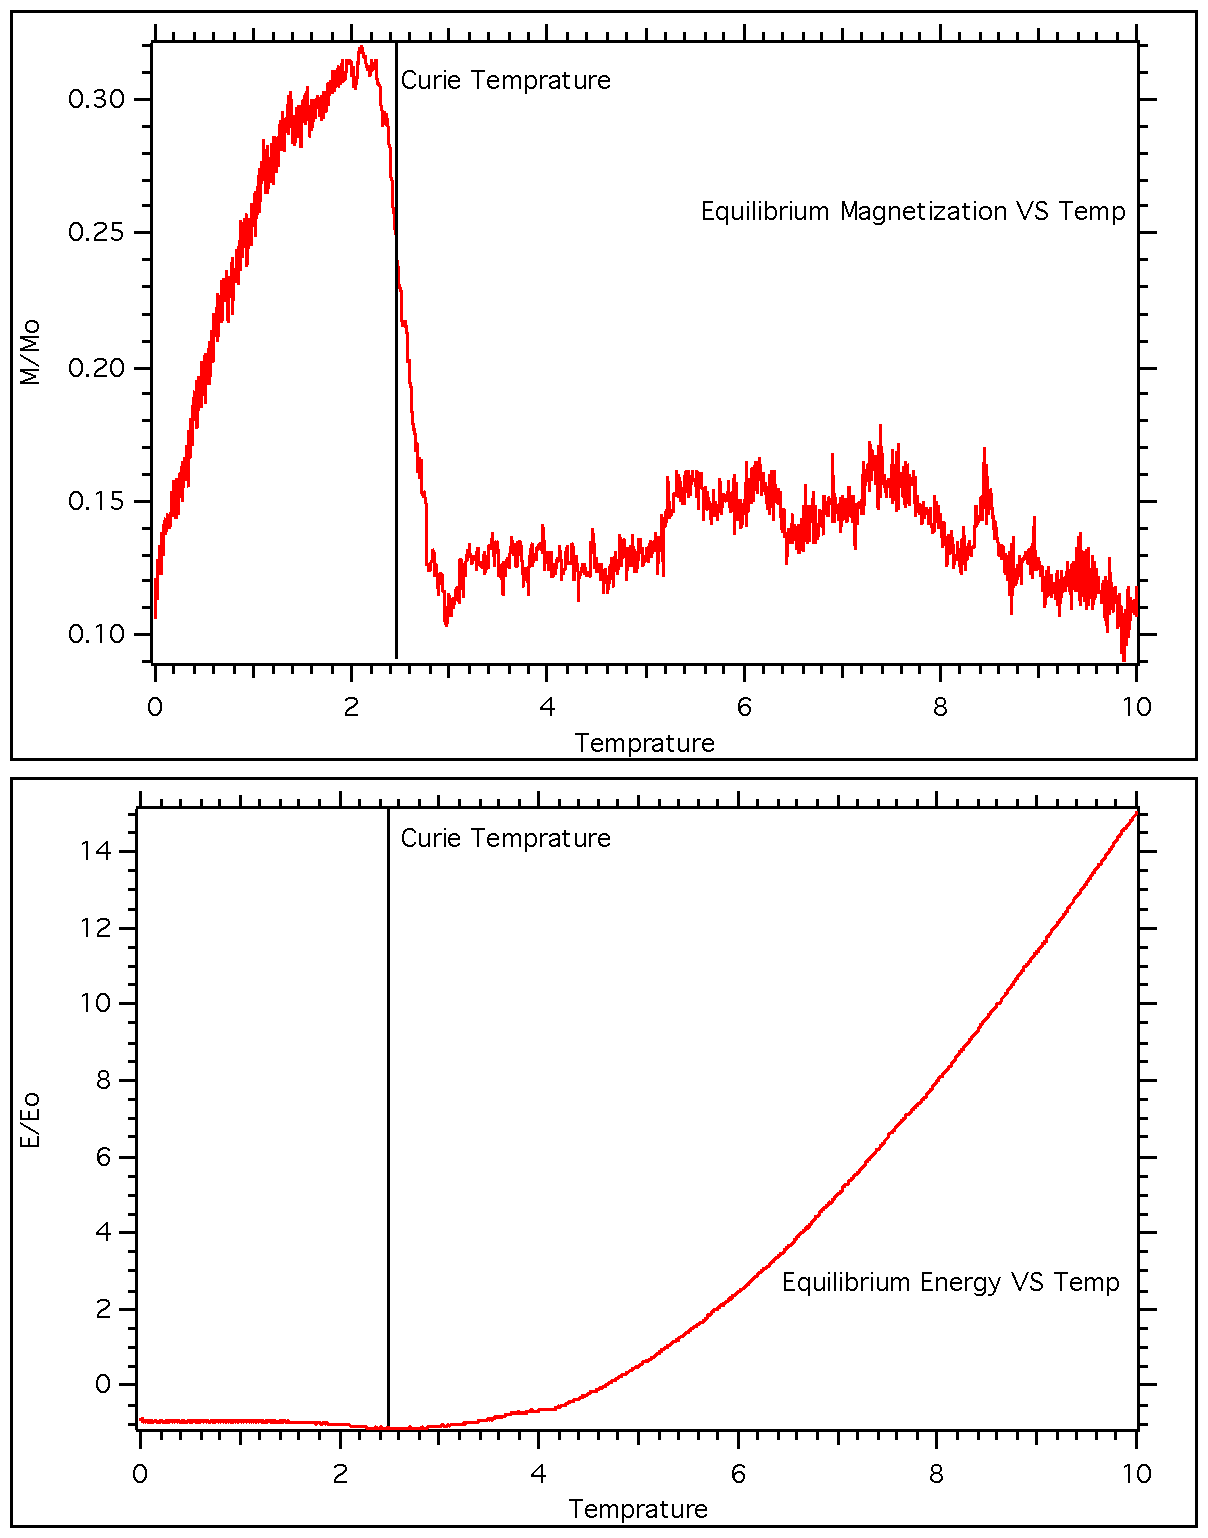
\includegraphics[width=0.5\textwidth]{Temp} \label{Temp}
  \end{figure}

We also ran test in which we observed the effects of temperature on normalized magnetisation and energy, as seen in fig~\ref{Temp}. From the graphs, we can see that as we increase the temperature, the normalised magnetisation approaches zero, and we can see a dramatic change near the curie temperature occurs in both the energy and the magnetisation graphs. 




After discussing the graph with Dr. Lindner, he pointed out to me that at low temperatures, the value of the normalised magnetisation should reach 1 as the magetisation should eventually be equal to the max magnetisation, as it is at lower temperatures that the electron's spins line up. However, I did not achieve this result for the low temperatures. Dr. Lindner suggested that I should wait for long times at the lower tempratures for the magnetic filed to freeze out ( for the majority of the spins to become constant), or maybe to change the boundary conditions of the program. However this turend to be more difficult than I thought it would be, hence I left the program as is.



      
   
  
%----------------------------------------------------------------------------------------


\end{document}